\documentclass[1p]{elsarticle_modified}
%\bibliographystyle{elsarticle-num}

%\usepackage[colorlinks]{hyperref}
%\usepackage{abbrmath_seonhwa} %\Abb, \Ascr, \Acal ,\Abf, \Afrak
\usepackage{amsfonts}
\usepackage{amssymb}
\usepackage{amsmath}
\usepackage{amsthm}
\usepackage{scalefnt}
\usepackage{amsbsy}
\usepackage{kotex}
\usepackage{caption}
\usepackage{subfig}
\usepackage{color}
\usepackage{graphicx}
\usepackage{xcolor} %% white, black, red, green, blue, cyan, magenta, yellow
\usepackage{float}
\usepackage{setspace}
\usepackage{hyperref}

\usepackage{tikz}
\usetikzlibrary{arrows}

\usepackage{multirow}
\usepackage{array} % fixed length table
\usepackage{hhline}

%%%%%%%%%%%%%%%%%%%%%
\makeatletter
\renewcommand*\env@matrix[1][\arraystretch]{%
	\edef\arraystretch{#1}%
	\hskip -\arraycolsep
	\let\@ifnextchar\new@ifnextchar
	\array{*\c@MaxMatrixCols c}}
\makeatother %https://tex.stackexchange.com/questions/14071/how-can-i-increase-the-line-spacing-in-a-matrix
%%%%%%%%%%%%%%%

\usepackage[normalem]{ulem}

\newcommand{\msout}[1]{\ifmmode\text{\sout{\ensuremath{#1}}}\else\sout{#1}\fi}
%SOURCE: \msout is \stkout macro in https://tex.stackexchange.com/questions/20609/strikeout-in-math-mode

\newcommand{\cancel}[1]{
	\ifmmode
	{\color{red}\msout{#1}}
	\else
	{\color{red}\sout{#1}}
	\fi
}

\newcommand{\add}[1]{
	{\color{blue}\uwave{#1}}
}

\newcommand{\replace}[2]{
	\ifmmode
	{\color{red}\msout{#1}}{\color{blue}\uwave{#2}}
	\else
	{\color{red}\sout{#1}}{\color{blue}\uwave{#2}}
	\fi
}

\newcommand{\Sol}{\mathcal{S}} %segment
\newcommand{\D}{D} %diagram
\newcommand{\A}{\mathcal{A}} %arc


%%%%%%%%%%%%%%%%%%%%%%%%%%%%%5 test

\def\sl{\operatorname{\textup{SL}}(2,\Cbb)}
\def\psl{\operatorname{\textup{PSL}}(2,\Cbb)}
\def\quan{\mkern 1mu \triangleright \mkern 1mu}

\theoremstyle{definition}
\newtheorem{thm}{Theorem}[section]
\newtheorem{prop}[thm]{Proposition}
\newtheorem{lem}[thm]{Lemma}
\newtheorem{ques}[thm]{Question}
\newtheorem{cor}[thm]{Corollary}
\newtheorem{defn}[thm]{Definition}
\newtheorem{exam}[thm]{Example}
\newtheorem{rmk}[thm]{Remark}
\newtheorem{alg}[thm]{Algorithm}

\newcommand{\I}{\sqrt{-1}}
\begin{document}

%\begin{frontmatter}
%
%\title{Boundary parabolic representations of knots up to 8 crossings}
%
%%% Group authors per affiliation:
%\author{Yunhi Cho} 
%\address{Department of Mathematics, University of Seoul, Seoul, Korea}
%\ead{yhcho@uos.ac.kr}
%
%
%\author{Seonhwa Kim} %\fnref{s_kim}}
%\address{Center for Geometry and Physics, Institute for Basic Science, Pohang, 37673, Korea}
%\ead{ryeona17@ibs.re.kr}
%
%\author{Hyuk Kim}
%\address{Department of Mathematical Sciences, Seoul National University, Seoul 08826, Korea}
%\ead{hyukkim@snu.ac.kr}
%
%\author{Seokbeom Yoon}
%\address{Department of Mathematical Sciences, Seoul National University, Seoul, 08826,  Korea}
%\ead{sbyoon15@snu.ac.kr}
%
%\begin{abstract}
%We find all boundary parabolic representation of knots up to 8 crossings.
%
%\end{abstract}
%\begin{keyword}
%    \MSC[2010] 57M25 
%\end{keyword}
%
%\end{frontmatter}

%\linenumbers
%\tableofcontents
%
\newcommand\colored[1]{\textcolor{white}{\rule[-0.35ex]{0.8em}{1.4ex}}\kern-0.8em\color{red} #1}%
%\newcommand\colored[1]{\textcolor{white}{ #1}\kern-2.17ex	\textcolor{white}{ #1}\kern-1.81ex	\textcolor{white}{ #1}\kern-2.15ex\color{red}#1	}

{\Large $\underline{11n_{60}~(K11n_{60})}$}

\setlength{\tabcolsep}{10pt}
\renewcommand{\arraystretch}{1.6}
\vspace{1cm}\begin{tabular}{m{100pt}>{\centering\arraybackslash}m{274pt}}
\multirow{5}{120pt}{
	\centering
	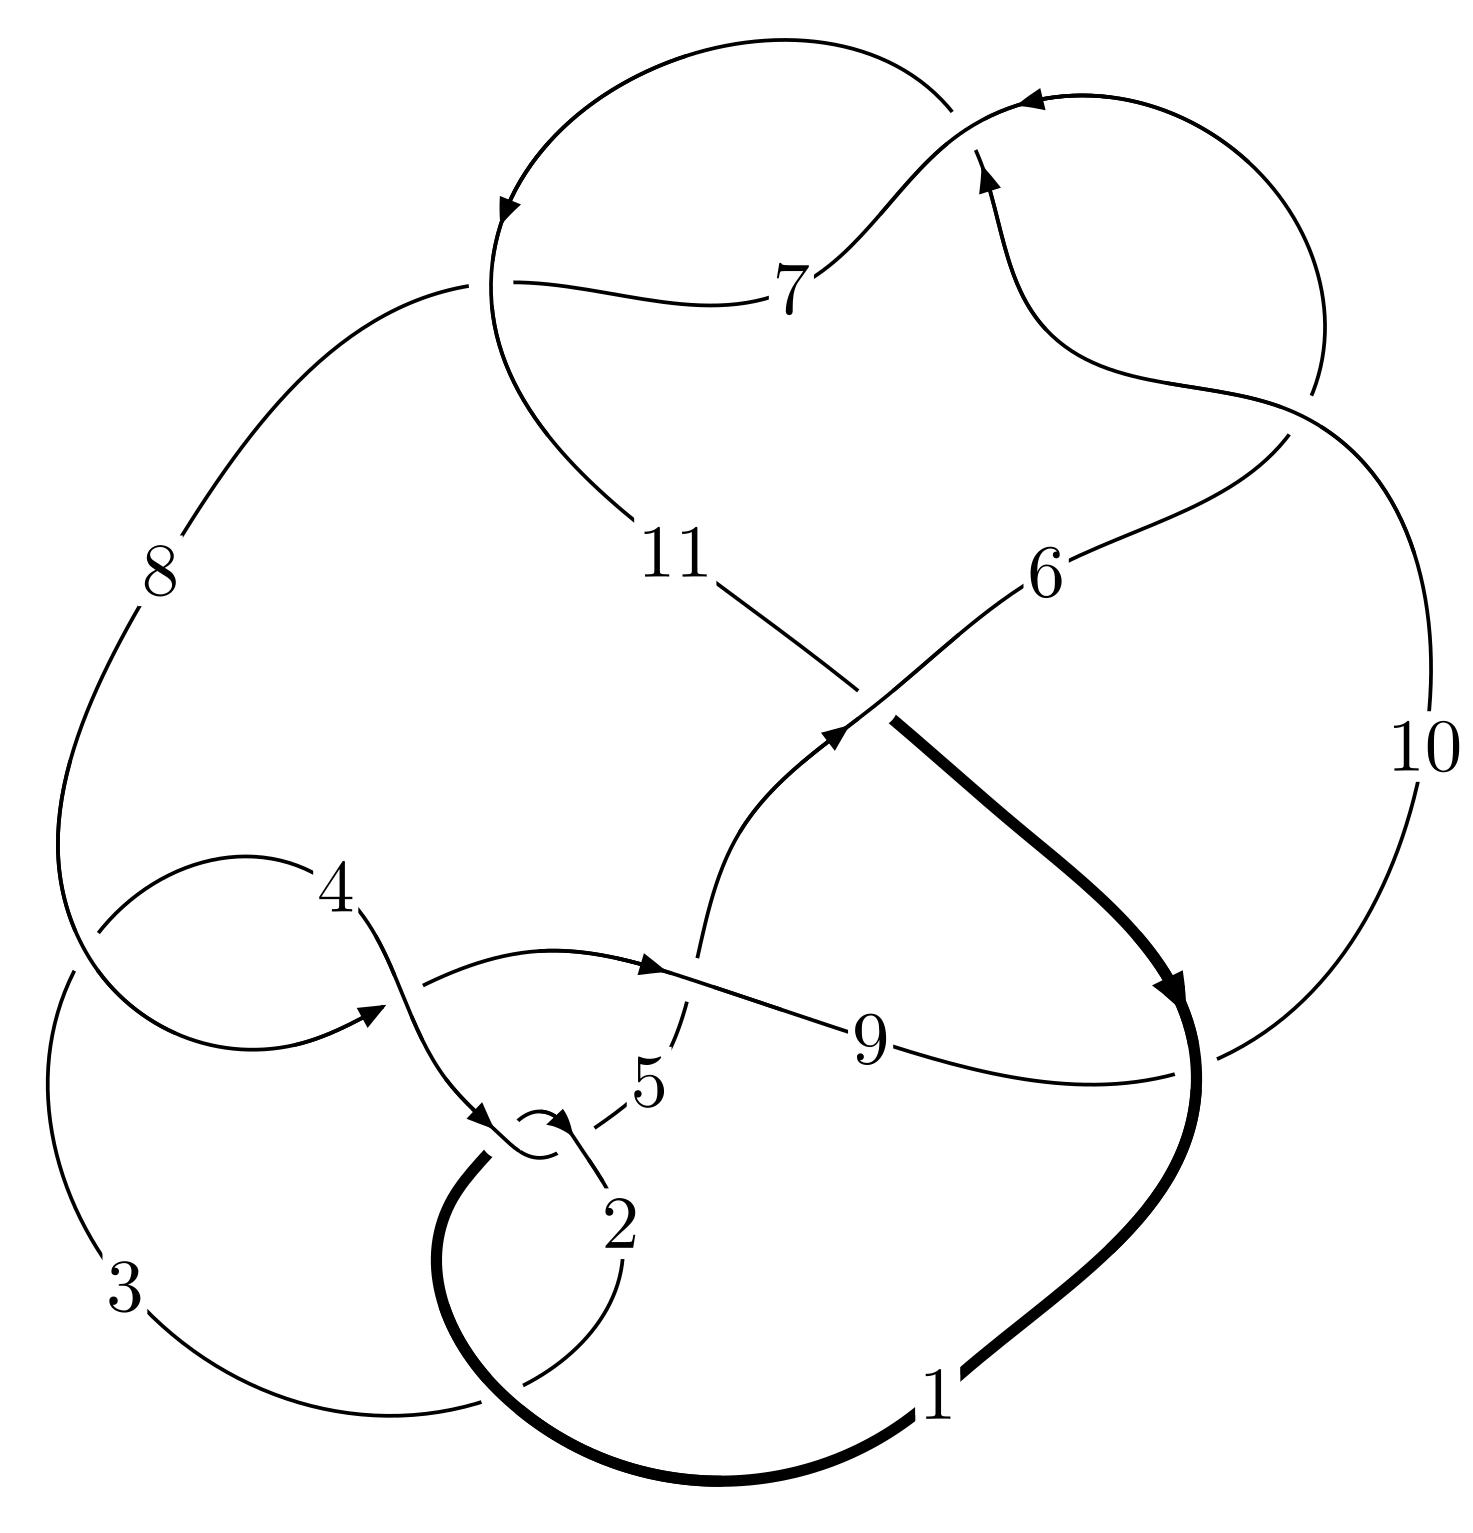
\includegraphics[width=112pt]{../../../GIT/diagram.site/Diagrams/png/676_11n_60.png}\\
\ \ \ A knot diagram\footnotemark}&
\allowdisplaybreaks
\textbf{Linearized knot diagam} \\
\cline{2-2}
 &
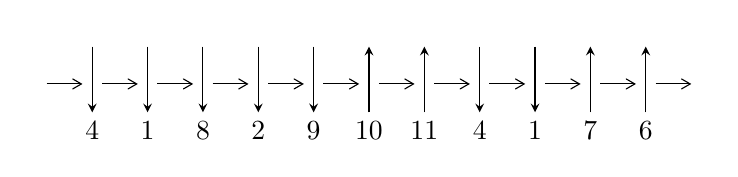
\begin{tikzpicture}[x=20pt, y=17pt]
	% nodes
	\node (C0) at (0, 0) {};
	\node (C1) at (1, 0) {};
	\node (C1U) at (1, +1) {};
	\node (C1D) at (1, -1) {4};

	\node (C2) at (2, 0) {};
	\node (C2U) at (2, +1) {};
	\node (C2D) at (2, -1) {1};

	\node (C3) at (3, 0) {};
	\node (C3U) at (3, +1) {};
	\node (C3D) at (3, -1) {8};

	\node (C4) at (4, 0) {};
	\node (C4U) at (4, +1) {};
	\node (C4D) at (4, -1) {2};

	\node (C5) at (5, 0) {};
	\node (C5U) at (5, +1) {};
	\node (C5D) at (5, -1) {9};

	\node (C6) at (6, 0) {};
	\node (C6U) at (6, +1) {};
	\node (C6D) at (6, -1) {10};

	\node (C7) at (7, 0) {};
	\node (C7U) at (7, +1) {};
	\node (C7D) at (7, -1) {11};

	\node (C8) at (8, 0) {};
	\node (C8U) at (8, +1) {};
	\node (C8D) at (8, -1) {4};

	\node (C9) at (9, 0) {};
	\node (C9U) at (9, +1) {};
	\node (C9D) at (9, -1) {1};

	\node (C10) at (10, 0) {};
	\node (C10U) at (10, +1) {};
	\node (C10D) at (10, -1) {7};

	\node (C11) at (11, 0) {};
	\node (C11U) at (11, +1) {};
	\node (C11D) at (11, -1) {6};
	\node (C12) at (12, 0) {};

	% arrows
	\draw[->,>={angle 60}]
	(C0) edge (C1) (C1) edge (C2) (C2) edge (C3) (C3) edge (C4) (C4) edge (C5) (C5) edge (C6) (C6) edge (C7) (C7) edge (C8) (C8) edge (C9) (C9) edge (C10) (C10) edge (C11) (C11) edge (C12) ;	\draw[->,>=stealth]
	(C1U) edge (C1D) (C2U) edge (C2D) (C3U) edge (C3D) (C4U) edge (C4D) (C5U) edge (C5D) (C6D) edge (C6U) (C7D) edge (C7U) (C8U) edge (C8D) (C9U) edge (C9D) (C10D) edge (C10U) (C11D) edge (C11U) ;
	\end{tikzpicture} \\
\hhline{~~} \\& 
\textbf{Solving Sequence} \\ \cline{2-2} 
 &
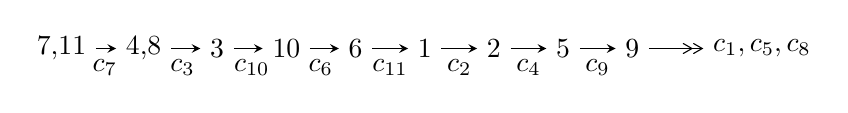
\begin{tikzpicture}[x=25pt, y=7pt]
	% node
	\node (A0) at (-1/8, 0) {7,11};
	\node (A1) at (17/16, 0) {4,8};
	\node (A2) at (17/8, 0) {3};
	\node (A3) at (25/8, 0) {10};
	\node (A4) at (33/8, 0) {6};
	\node (A5) at (41/8, 0) {1};
	\node (A6) at (49/8, 0) {2};
	\node (A7) at (57/8, 0) {5};
	\node (A8) at (65/8, 0) {9};
	\node (C1) at (1/2, -1) {$c_{7}$};
	\node (C2) at (13/8, -1) {$c_{3}$};
	\node (C3) at (21/8, -1) {$c_{10}$};
	\node (C4) at (29/8, -1) {$c_{6}$};
	\node (C5) at (37/8, -1) {$c_{11}$};
	\node (C6) at (45/8, -1) {$c_{2}$};
	\node (C7) at (53/8, -1) {$c_{4}$};
	\node (C8) at (61/8, -1) {$c_{9}$};
	\node (A9) at (10, 0) {$c_{1},c_{5},c_{8}$};

	% edge
	\draw[->,>=stealth]	
	(A0) edge (A1) (A1) edge (A2) (A2) edge (A3) (A3) edge (A4) (A4) edge (A5) (A5) edge (A6) (A6) edge (A7) (A7) edge (A8) ;
	\draw[->>,>={angle 60}]	
	(A8) edge (A9);
\end{tikzpicture} \\ 

\end{tabular} \\

\footnotetext{
The image of knot diagram is generated by the software ``\textbf{Draw programme}" developed by Andrew Bartholomew(\url{http://www.layer8.co.uk/maths/draw/index.htm\#Running-draw}), where we modified some parts for our purpose(\url{https://github.com/CATsTAILs/LinksPainter}).
}\phantom \\ \newline 
\centering \textbf{Ideals for irreducible components\footnotemark of $X_{\text{par}}$} 
 
\begin{align*}
I^u_{1}&=\langle 
2 u^{19}+u^{18}+\cdots+b-2,\;u^{18}+u^{17}+\cdots+a+2,\;u^{20}+2 u^{19}+\cdots+3 u-1\rangle \\
I^u_{2}&=\langle 
u^4- u^2+b- u,\;- u^4+u^3+u^2+a- u,\;u^5- u^4-2 u^3+u^2+u+1\rangle \\
\\
\end{align*}
\raggedright * 2 irreducible components of $\dim_{\mathbb{C}}=0$, with total 25 representations.\\
\footnotetext{All coefficients of polynomials are rational numbers. But the coefficients are sometimes approximated in decimal forms when there is not enough margin.}
\newpage
\renewcommand{\arraystretch}{1}
\centering \section*{I. $I^u_{1}= \langle 2 u^{19}+u^{18}+\cdots+b-2,\;u^{18}+u^{17}+\cdots+a+2,\;u^{20}+2 u^{19}+\cdots+3 u-1 \rangle$}
\flushleft \textbf{(i) Arc colorings}\\
\begin{tabular}{m{7pt} m{180pt} m{7pt} m{180pt} }
\flushright $a_{7}=$&$\begin{pmatrix}1\\0\end{pmatrix}$ \\
\flushright $a_{11}=$&$\begin{pmatrix}0\\u\end{pmatrix}$ \\
\flushright $a_{4}=$&$\begin{pmatrix}- u^{18}- u^{17}+\cdots-5 u^2-2\\-2 u^{19}- u^{18}+\cdots-5 u+2\end{pmatrix}$ \\
\flushright $a_{8}=$&$\begin{pmatrix}1\\- u^2\end{pmatrix}$ \\
\flushright $a_{3}=$&$\begin{pmatrix}- u^{19}- u^{18}+\cdots-2 u-1\\u^{19}+u^{18}+\cdots+u^2+2 u\end{pmatrix}$ \\
\flushright $a_{10}=$&$\begin{pmatrix}- u\\u\end{pmatrix}$ \\
\flushright $a_{6}=$&$\begin{pmatrix}- u^2+1\\u^2\end{pmatrix}$ \\
\flushright $a_{1}=$&$\begin{pmatrix}u^5-2 u^3+u\\- u^5+u^3+u\end{pmatrix}$ \\
\flushright $a_{2}=$&$\begin{pmatrix}- u^{18}- u^{17}+\cdots- u-1\\- u^{19}+8 u^{17}+\cdots- u+1\end{pmatrix}$ \\
\flushright $a_{5}=$&$\begin{pmatrix}- u^{16}+7 u^{14}-19 u^{12}+24 u^{10}-13 u^8+2 u^6-1\\u^{16}-6 u^{14}+12 u^{12}-6 u^{10}-6 u^8+2 u^6+4 u^4\end{pmatrix}$ \\
\flushright $a_{9}=$&$\begin{pmatrix}- u^9+4 u^7-5 u^5+2 u^3- u\\u^9-3 u^7+u^5+2 u^3+u\end{pmatrix}$\\ \flushright $a_{9}=$&$\begin{pmatrix}- u^9+4 u^7-5 u^5+2 u^3- u\\u^9-3 u^7+u^5+2 u^3+u\end{pmatrix}$\\&\end{tabular}
\flushleft \textbf{(ii) Obstruction class $= -1$}\\~\\
\flushleft \textbf{(iii) Cusp Shapes $= 2 u^{19}-16 u^{17}+3 u^{16}+49 u^{15}-22 u^{14}-61 u^{13}+58 u^{12}-8 u^{11}-54 u^{10}+91 u^9-20 u^8-50 u^7+52 u^6-40 u^5+26 u^3-12 u^2+9 u-10$}\\~\\
\newpage\renewcommand{\arraystretch}{1}
\flushleft \textbf{(iv) u-Polynomials at the component}\newline \\
\begin{tabular}{m{50pt}|m{274pt}}
Crossings & \hspace{64pt}u-Polynomials at each crossing \\
\hline $$\begin{aligned}c_{1},c_{4}\end{aligned}$$&$\begin{aligned}
&u^{20}-6 u^{19}+\cdots+7 u-1
\end{aligned}$\\
\hline $$\begin{aligned}c_{2}\end{aligned}$$&$\begin{aligned}
&u^{20}+30 u^{19}+\cdots+13 u+1
\end{aligned}$\\
\hline $$\begin{aligned}c_{3},c_{8}\end{aligned}$$&$\begin{aligned}
&u^{20}- u^{19}+\cdots+32 u+32
\end{aligned}$\\
\hline $$\begin{aligned}c_{5}\end{aligned}$$&$\begin{aligned}
&u^{20}+2 u^{19}+\cdots-3 u-1
\end{aligned}$\\
\hline $$\begin{aligned}c_{6},c_{7},c_{10}\end{aligned}$$&$\begin{aligned}
&u^{20}-2 u^{19}+\cdots-3 u-1
\end{aligned}$\\
\hline $$\begin{aligned}c_{9}\end{aligned}$$&$\begin{aligned}
&u^{20}-6 u^{19}+\cdots+81 u-9
\end{aligned}$\\
\hline $$\begin{aligned}c_{11}\end{aligned}$$&$\begin{aligned}
&u^{20}+6 u^{19}+\cdots+35 u+5
\end{aligned}$\\
\hline
\end{tabular}\\~\\
\newpage\renewcommand{\arraystretch}{1}
\flushleft \textbf{(v) Riley Polynomials at the component}\newline \\
\begin{tabular}{m{50pt}|m{274pt}}
Crossings & \hspace{64pt}Riley Polynomials at each crossing \\
\hline $$\begin{aligned}c_{1},c_{4}\end{aligned}$$&$\begin{aligned}
&y^{20}-30 y^{19}+\cdots-13 y+1
\end{aligned}$\\
\hline $$\begin{aligned}c_{2}\end{aligned}$$&$\begin{aligned}
&y^{20}-74 y^{19}+\cdots+355 y+1
\end{aligned}$\\
\hline $$\begin{aligned}c_{3},c_{8}\end{aligned}$$&$\begin{aligned}
&y^{20}-33 y^{19}+\cdots+3584 y+1024
\end{aligned}$\\
\hline $$\begin{aligned}c_{5}\end{aligned}$$&$\begin{aligned}
&y^{20}-42 y^{19}+\cdots-11 y+1
\end{aligned}$\\
\hline $$\begin{aligned}c_{6},c_{7},c_{10}\end{aligned}$$&$\begin{aligned}
&y^{20}-18 y^{19}+\cdots-11 y+1
\end{aligned}$\\
\hline $$\begin{aligned}c_{9}\end{aligned}$$&$\begin{aligned}
&y^{20}-6 y^{19}+\cdots-5031 y+81
\end{aligned}$\\
\hline $$\begin{aligned}c_{11}\end{aligned}$$&$\begin{aligned}
&y^{20}+6 y^{19}+\cdots-335 y+25
\end{aligned}$\\
\hline
\end{tabular}\\~\\
\newpage\flushleft \textbf{(vi) Complex Volumes and Cusp Shapes}
$$\begin{array}{c|c|c}  
\text{Solutions to }I^u_{1}& \I (\text{vol} + \sqrt{-1}CS) & \text{Cusp shape}\\
 \hline 
\begin{aligned}
u &= \phantom{-}0.917550 + 0.464269 I \\
a &= \phantom{-}0.887708 + 0.822675 I \\
b &= -2.03002 - 1.48307 I\end{aligned}
 & -12.36330 - 0.65965 I & -5.32167 - 1.11773 I \\ \hline\begin{aligned}
u &= \phantom{-}0.917550 - 0.464269 I \\
a &= \phantom{-}0.887708 - 0.822675 I \\
b &= -2.03002 + 1.48307 I\end{aligned}
 & -12.36330 + 0.65965 I & -5.32167 + 1.11773 I \\ \hline\begin{aligned}
u &= \phantom{-}0.243336 + 0.826957 I \\
a &= -2.56703 - 1.06992 I \\
b &= \phantom{-}0.1190440 - 0.0724083 I\end{aligned}
 & -14.4810 + 5.2607 I & -7.68359 - 3.29127 I \\ \hline\begin{aligned}
u &= \phantom{-}0.243336 - 0.826957 I \\
a &= -2.56703 + 1.06992 I \\
b &= \phantom{-}0.1190440 + 0.0724083 I\end{aligned}
 & -14.4810 - 5.2607 I & -7.68359 + 3.29127 I \\ \hline\begin{aligned}
u &= \phantom{-}1.238020 + 0.241187 I \\
a &= -1.48735 - 1.05770 I \\
b &= \phantom{-}2.32454 + 1.44360 I\end{aligned}
 & -0.14678 + 1.84866 I & -3.98019 - 2.83860 I \\ \hline\begin{aligned}
u &= \phantom{-}1.238020 - 0.241187 I \\
a &= -1.48735 + 1.05770 I \\
b &= \phantom{-}2.32454 - 1.44360 I\end{aligned}
 & -0.14678 - 1.84866 I & -3.98019 + 2.83860 I \\ \hline\begin{aligned}
u &= -1.278360 + 0.104707 I \\
a &= \phantom{-}0.191843 - 0.012837 I \\
b &= -1.001270 + 0.473795 I\end{aligned}
 & \phantom{-}3.00168 - 0.46375 I & \phantom{-}0.380412 - 0.924408 I \\ \hline\begin{aligned}
u &= -1.278360 - 0.104707 I \\
a &= \phantom{-}0.191843 + 0.012837 I \\
b &= -1.001270 - 0.473795 I\end{aligned}
 & \phantom{-}3.00168 + 0.46375 I & \phantom{-}0.380412 + 0.924408 I \\ \hline\begin{aligned}
u &= \phantom{-}0.069392 + 0.685215 I \\
a &= \phantom{-}2.21387 + 0.78494 I \\
b &= \phantom{-}0.040683 - 0.477218 I\end{aligned}
 & -3.69282 + 1.48185 I & -9.31815 - 1.78036 I \\ \hline\begin{aligned}
u &= \phantom{-}0.069392 - 0.685215 I \\
a &= \phantom{-}2.21387 - 0.78494 I \\
b &= \phantom{-}0.040683 + 0.477218 I\end{aligned}
 & -3.69282 - 1.48185 I & -9.31815 + 1.78036 I\\
 \hline 
 \end{array}$$\newpage$$\begin{array}{c|c|c}  
\text{Solutions to }I^u_{1}& \I (\text{vol} + \sqrt{-1}CS) & \text{Cusp shape}\\
 \hline 
\begin{aligned}
u &= -1.314810 + 0.281063 I \\
a &= -0.578126 + 0.956901 I \\
b &= \phantom{-}1.58117 - 2.41766 I\end{aligned}
 & \phantom{-}0.65473 - 4.99045 I & -3.53301 + 4.53534 I \\ \hline\begin{aligned}
u &= -1.314810 - 0.281063 I \\
a &= -0.578126 - 0.956901 I \\
b &= \phantom{-}1.58117 + 2.41766 I\end{aligned}
 & \phantom{-}0.65473 + 4.99045 I & -3.53301 - 4.53534 I \\ \hline\begin{aligned}
u &= \phantom{-}1.39777 + 0.21985 I \\
a &= \phantom{-}0.535073 + 0.493687 I \\
b &= -0.802086 - 0.653876 I\end{aligned}
 & \phantom{-}5.26329 + 4.10687 I & \phantom{-}5.09324 - 3.12286 I \\ \hline\begin{aligned}
u &= \phantom{-}1.39777 - 0.21985 I \\
a &= \phantom{-}0.535073 - 0.493687 I \\
b &= -0.802086 + 0.653876 I\end{aligned}
 & \phantom{-}5.26329 - 4.10687 I & \phantom{-}5.09324 + 3.12286 I \\ \hline\begin{aligned}
u &= -0.243428 + 0.530766 I \\
a &= -0.710922 - 0.053518 I \\
b &= \phantom{-}0.009442 + 0.295836 I\end{aligned}
 & \phantom{-}0.003151 - 1.284380 I & -0.00392 + 4.85690 I \\ \hline\begin{aligned}
u &= -0.243428 - 0.530766 I \\
a &= -0.710922 + 0.053518 I \\
b &= \phantom{-}0.009442 - 0.295836 I\end{aligned}
 & \phantom{-}0.003151 + 1.284380 I & -0.00392 - 4.85690 I \\ \hline\begin{aligned}
u &= -1.41087 + 0.34270 I \\
a &= \phantom{-}0.67202 - 2.01481 I \\
b &= -1.37414 + 3.84768 I\end{aligned}
 & -9.22640 - 9.48716 I & -3.68120 + 4.58970 I \\ \hline\begin{aligned}
u &= -1.41087 - 0.34270 I \\
a &= \phantom{-}0.67202 + 2.01481 I \\
b &= -1.37414 - 3.84768 I\end{aligned}
 & -9.22640 + 9.48716 I & -3.68120 - 4.58970 I \\ \hline\begin{aligned}
u &= -1.49993\phantom{ +0.000000I} \\
a &= \phantom{-}0.998510\phantom{ +0.000000I} \\
b &= -0.427242\phantom{ +0.000000I}\end{aligned}
 & -4.28328\phantom{ +0.000000I} & -1.87430\phantom{ +0.000000I} \\ \hline\begin{aligned}
u &= \phantom{-}0.262728\phantom{ +0.000000I} \\
a &= -2.31269\phantom{ +0.000000I} \\
b &= \phantom{-}0.692511\phantom{ +0.000000I}\end{aligned}
 & -1.18420\phantom{ +0.000000I} & -8.02950\phantom{ +0.000000I}\\
 \hline 
 \end{array}$$\newpage\newpage\renewcommand{\arraystretch}{1}
\centering \section*{II. $I^u_{2}= \langle u^4- u^2+b- u,\;- u^4+u^3+u^2+a- u,\;u^5- u^4-2 u^3+u^2+u+1 \rangle$}
\flushleft \textbf{(i) Arc colorings}\\
\begin{tabular}{m{7pt} m{180pt} m{7pt} m{180pt} }
\flushright $a_{7}=$&$\begin{pmatrix}1\\0\end{pmatrix}$ \\
\flushright $a_{11}=$&$\begin{pmatrix}0\\u\end{pmatrix}$ \\
\flushright $a_{4}=$&$\begin{pmatrix}u^4- u^3- u^2+u\\- u^4+u^2+u\end{pmatrix}$ \\
\flushright $a_{8}=$&$\begin{pmatrix}1\\- u^2\end{pmatrix}$ \\
\flushright $a_{3}=$&$\begin{pmatrix}u^4- u^3- u^2+u\\- u^4+u^2+u\end{pmatrix}$ \\
\flushright $a_{10}=$&$\begin{pmatrix}- u\\u\end{pmatrix}$ \\
\flushright $a_{6}=$&$\begin{pmatrix}- u^2+1\\u^2\end{pmatrix}$ \\
\flushright $a_{1}=$&$\begin{pmatrix}u^4- u^2-1\\- u^4- u^3+u^2+2 u+1\end{pmatrix}$ \\
\flushright $a_{2}=$&$\begin{pmatrix}2 u^4- u^3-2 u^2+u-1\\-2 u^4- u^3+2 u^2+3 u+1\end{pmatrix}$ \\
\flushright $a_{5}=$&$\begin{pmatrix}- u^4+u^2+1\\u^4+u^3- u^2-2 u-1\end{pmatrix}$ \\
\flushright $a_{9}=$&$\begin{pmatrix}1\\- u^2\end{pmatrix}$\\ \flushright $a_{9}=$&$\begin{pmatrix}1\\- u^2\end{pmatrix}$\\&\end{tabular}
\flushleft \textbf{(ii) Obstruction class $= 1$}\\~\\
\flushleft \textbf{(iii) Cusp Shapes $= -5 u^3+u^2+8 u-3$}\\~\\
\newpage\renewcommand{\arraystretch}{1}
\flushleft \textbf{(iv) u-Polynomials at the component}\newline \\
\begin{tabular}{m{50pt}|m{274pt}}
Crossings & \hspace{64pt}u-Polynomials at each crossing \\
\hline $$\begin{aligned}c_{1}\end{aligned}$$&$\begin{aligned}
&(u-1)^5
\end{aligned}$\\
\hline $$\begin{aligned}c_{2},c_{4}\end{aligned}$$&$\begin{aligned}
&(u+1)^5
\end{aligned}$\\
\hline $$\begin{aligned}c_{3},c_{8}\end{aligned}$$&$\begin{aligned}
&u^5
\end{aligned}$\\
\hline $$\begin{aligned}c_{5},c_{9}\end{aligned}$$&$\begin{aligned}
&u^5+u^4+2 u^3+u^2+u+1
\end{aligned}$\\
\hline $$\begin{aligned}c_{6},c_{7}\end{aligned}$$&$\begin{aligned}
&u^5- u^4-2 u^3+u^2+u+1
\end{aligned}$\\
\hline $$\begin{aligned}c_{10}\end{aligned}$$&$\begin{aligned}
&u^5+u^4-2 u^3- u^2+u-1
\end{aligned}$\\
\hline $$\begin{aligned}c_{11}\end{aligned}$$&$\begin{aligned}
&u^5-3 u^4+4 u^3- u^2- u+1
\end{aligned}$\\
\hline
\end{tabular}\\~\\
\newpage\renewcommand{\arraystretch}{1}
\flushleft \textbf{(v) Riley Polynomials at the component}\newline \\
\begin{tabular}{m{50pt}|m{274pt}}
Crossings & \hspace{64pt}Riley Polynomials at each crossing \\
\hline $$\begin{aligned}c_{1},c_{2},c_{4}\end{aligned}$$&$\begin{aligned}
&(y-1)^5
\end{aligned}$\\
\hline $$\begin{aligned}c_{3},c_{8}\end{aligned}$$&$\begin{aligned}
&y^5
\end{aligned}$\\
\hline $$\begin{aligned}c_{5},c_{9}\end{aligned}$$&$\begin{aligned}
&y^5+3 y^4+4 y^3+y^2- y-1
\end{aligned}$\\
\hline $$\begin{aligned}c_{6},c_{7},c_{10}\end{aligned}$$&$\begin{aligned}
&y^5-5 y^4+8 y^3-3 y^2- y-1
\end{aligned}$\\
\hline $$\begin{aligned}c_{11}\end{aligned}$$&$\begin{aligned}
&y^5- y^4+8 y^3-3 y^2+3 y-1
\end{aligned}$\\
\hline
\end{tabular}\\~\\
\newpage\flushleft \textbf{(vi) Complex Volumes and Cusp Shapes}
$$\begin{array}{c|c|c}  
\text{Solutions to }I^u_{2}& \I (\text{vol} + \sqrt{-1}CS) & \text{Cusp shape}\\
 \hline 
\begin{aligned}
u &= -1.21774\phantom{ +0.000000I} \\
a &= \phantom{-}1.30408\phantom{ +0.000000I} \\
b &= -1.93379\phantom{ +0.000000I}\end{aligned}
 & \phantom{-}0.756147\phantom{ +0.000000I} & -2.23020\phantom{ +0.000000I} \\ \hline\begin{aligned}
u &= -0.309916 + 0.549911 I \\
a &= -0.428550 + 1.039280 I \\
b &= -0.442672 + 0.068387 I\end{aligned}
 & -1.31583 - 1.53058 I & -6.94263 + 4.09764 I \\ \hline\begin{aligned}
u &= -0.309916 - 0.549911 I \\
a &= -0.428550 - 1.039280 I \\
b &= -0.442672 - 0.068387 I\end{aligned}
 & -1.31583 + 1.53058 I & -6.94263 - 4.09764 I \\ \hline\begin{aligned}
u &= \phantom{-}1.41878 + 0.21917 I \\
a &= \phantom{-}0.276511 + 0.728237 I \\
b &= -0.09043 - 1.60288 I\end{aligned}
 & \phantom{-}4.22763 + 4.40083 I & -2.94226 - 4.18967 I \\ \hline\begin{aligned}
u &= \phantom{-}1.41878 - 0.21917 I \\
a &= \phantom{-}0.276511 - 0.728237 I \\
b &= -0.09043 + 1.60288 I\end{aligned}
 & \phantom{-}4.22763 - 4.40083 I & -2.94226 + 4.18967 I\\
 \hline 
 \end{array}$$\newpage
\newpage\renewcommand{\arraystretch}{1}
\centering \section*{ III. u-Polynomials}
\begin{tabular}{m{50pt}|m{274pt}}
Crossings & \hspace{64pt}u-Polynomials at each crossing \\
\hline $$\begin{aligned}c_{1}\end{aligned}$$&$\begin{aligned}
&((u-1)^5)(u^{20}-6 u^{19}+\cdots+7 u-1)
\end{aligned}$\\
\hline $$\begin{aligned}c_{2}\end{aligned}$$&$\begin{aligned}
&((u+1)^5)(u^{20}+30 u^{19}+\cdots+13 u+1)
\end{aligned}$\\
\hline $$\begin{aligned}c_{3},c_{8}\end{aligned}$$&$\begin{aligned}
&u^5(u^{20}- u^{19}+\cdots+32 u+32)
\end{aligned}$\\
\hline $$\begin{aligned}c_{4}\end{aligned}$$&$\begin{aligned}
&((u+1)^5)(u^{20}-6 u^{19}+\cdots+7 u-1)
\end{aligned}$\\
\hline $$\begin{aligned}c_{5}\end{aligned}$$&$\begin{aligned}
&(u^5+u^4+2 u^3+u^2+u+1)(u^{20}+2 u^{19}+\cdots-3 u-1)
\end{aligned}$\\
\hline $$\begin{aligned}c_{6},c_{7}\end{aligned}$$&$\begin{aligned}
&(u^5- u^4-2 u^3+u^2+u+1)(u^{20}-2 u^{19}+\cdots-3 u-1)
\end{aligned}$\\
\hline $$\begin{aligned}c_{9}\end{aligned}$$&$\begin{aligned}
&(u^5+u^4+2 u^3+u^2+u+1)(u^{20}-6 u^{19}+\cdots+81 u-9)
\end{aligned}$\\
\hline $$\begin{aligned}c_{10}\end{aligned}$$&$\begin{aligned}
&(u^5+u^4-2 u^3- u^2+u-1)(u^{20}-2 u^{19}+\cdots-3 u-1)
\end{aligned}$\\
\hline $$\begin{aligned}c_{11}\end{aligned}$$&$\begin{aligned}
&(u^5-3 u^4+4 u^3- u^2- u+1)(u^{20}+6 u^{19}+\cdots+35 u+5)
\end{aligned}$\\
\hline
\end{tabular}\newpage\renewcommand{\arraystretch}{1}
\centering \section*{ IV. Riley Polynomials}
\begin{tabular}{m{50pt}|m{274pt}}
Crossings & \hspace{64pt}Riley Polynomials at each crossing \\
\hline $$\begin{aligned}c_{1},c_{4}\end{aligned}$$&$\begin{aligned}
&((y-1)^5)(y^{20}-30 y^{19}+\cdots-13 y+1)
\end{aligned}$\\
\hline $$\begin{aligned}c_{2}\end{aligned}$$&$\begin{aligned}
&((y-1)^5)(y^{20}-74 y^{19}+\cdots+355 y+1)
\end{aligned}$\\
\hline $$\begin{aligned}c_{3},c_{8}\end{aligned}$$&$\begin{aligned}
&y^5(y^{20}-33 y^{19}+\cdots+3584 y+1024)
\end{aligned}$\\
\hline $$\begin{aligned}c_{5}\end{aligned}$$&$\begin{aligned}
&(y^5+3 y^4+4 y^3+y^2- y-1)(y^{20}-42 y^{19}+\cdots-11 y+1)
\end{aligned}$\\
\hline $$\begin{aligned}c_{6},c_{7},c_{10}\end{aligned}$$&$\begin{aligned}
&(y^5-5 y^4+8 y^3-3 y^2- y-1)(y^{20}-18 y^{19}+\cdots-11 y+1)
\end{aligned}$\\
\hline $$\begin{aligned}c_{9}\end{aligned}$$&$\begin{aligned}
&(y^5+3 y^4+4 y^3+y^2- y-1)(y^{20}-6 y^{19}+\cdots-5031 y+81)
\end{aligned}$\\
\hline $$\begin{aligned}c_{11}\end{aligned}$$&$\begin{aligned}
&(y^5- y^4+8 y^3-3 y^2+3 y-1)(y^{20}+6 y^{19}+\cdots-335 y+25)
\end{aligned}$\\
\hline
\end{tabular}
\vskip 2pc
\end{document}